%---------------------------------------------------------------------------- 
\chapter{Hívásfelépítés Kubernetes nélkül}
%---------------------------------------------------------------------------- 



\section{rtpengine}



\section{Kamailio}

A Kamailio egy SIP Signaling Server nyílt forráskódú megvalósítása. Amit nagy rendszerek
skálázhatóságára terveztek, de használható cégek és egyének számára is.

A használatához általában szükség van valamilyen Kamailio által támogatott adatbázishoz,
de elméletileg lehet adatbázis nélkül is használni, de akkor elvesztünk bizonyos funkciókat. 
Ezért az ajánlott adatbázist használtam hozzá, ami egy lokálisan futó mysql szerver. Ebbe 
az adatbázisba olyan táblákat tárol, mint regisztrált felhasználók és aktív hívások, de 
ezen felül még sok mást is. 

Ezenkívül az általam használt beállításokat a \textit{kamailio.cfg} fájlban lehet megadni,
ami három részből áll. A használt dokumentációból \cite{kamailio} jól látszik, hogy ennek
fájlnak a szerkesztése nagyon sok szempontból emlékeztet egy programozási nyelvre 
C szerű elemekkel.  

Az első a \textbf{globális paraméterek}, ahol leginkább környezeti változókat lehet 
definiálni, amikkel lehet kontrollálni, hogy a konfiguráció mely része fusson le illetve
értékeket is lehet hozzájuk rendelni. 

Aztán jönnek a \textbf{modul beállítások}, ahol az alapértelmezett modulokhoz tudunk plusz
modulokat betölteni és beállítani. Ez azért egy fontos rész, mert a Kamailio alapvetően 
nem rtpengine-re van beállítva, hanem annak az előző verziójához, ami az rtpproxy. Ami 
nem kerül telepítésre az kamailio-val együtt. Így, ha se rtpengine se rtpproxy nincs,
akkor az kamailio két SIP klienst közvetlen fogja összekötni.

Végül van az \textbf{irányítási blokk}, ahol különböző SIP üzenetekre lehet megmondani, hogy mi
történjen velük, ha beérkeznek a hálózati interfészre. Itt betudjuk állítani azt, hogy
az \textbf{INVITE} üzenetek esetén az ng vezérlőprotokollon keresztül állítsa be a hívást
az rtpengine szerveren.

\section{Kommunikáció}

Az normál architektúrához a már említett VirtualBox-l létrehoztam négy virtuális gépet,
amik Ubuntu 20.04 operációs rendszer használnak. Ezek közül egyre telepítésre került 
a Kamailio, egyre az rtpengine és kettőre egy-egy Linphone kliens. A klienseknek azért
van szüksége két különböző virtuális gépre, mert Linphone-ból nem lehet kettőt
párhuzamosan futtatni egy gépen.

A Kamailio beállítása során egy a publikus Github tárolóban található konfigurációt
használtam, mivel abban beállításra került az rtpengine használata. Így nekem 
csak a modul inicializáció során kellett megadnom az rtpengine címét és annak portját. 
Viszont az rtpengine beállítása teljes mértékben azonos a \ref{lst:confRtpe} megadott konfigurációval azzal a különbséggel, hogy más IP címek szerepelnek benne.

Amit még a Kamailio-val kellett tenni, hogy két felhasználókat kellett regisztrálni
különben nem lehetne a két kliens között hívást kezdeményezni. Az ehhez használt parancs
az \ref{lst:addUserKamailio} látható, ahol az első paraméter a felhasználó neve majd az azutáni a felhasználó jelszava.

\begin{lstlisting}[caption=Felhasználó hozzáadása Kamailio-hoz, label=lst:addUserKamailio]
kamctl add A 123
\end{lstlisting}

Abban az esetben, ha a Kamailio-t futtató szerver IP címe 192.168.99.102, akkor az 
így létrejött felhasználó azonosítója a következő lesz: sip:A@192.168.99.102. Ezzel a
címmel lehet a Linphone kliensekben regisztrálni ezt a felhasználót. 

De hogyan is kell beállítani a Linphone klienseket? Erre add választ a következő 
pár sor. 

\begin{lstlisting}[caption=Linphone beállítása, label=lst:setupLinphone]
register sip:A@192.168.99.102 192.168.99.102 123
soundcard use files
play /home/user/input.wan
\end{lstlisting}

Az első sorral kerül regisztrálásra a felhasználó, ahol az első argumentum adja meg a 
felhasználó azonosítóját, második a tartomány címét és a végül a jelszó kerül átadásra. 
Ezután, ha újraindításra kerül a Linphone, akkor automatikusan megpróbálja a definiált
felhasználót regisztrálni. 

A következő sor azt adja meg, hogy ne használjon semmilyen hangkártyát és csak a 
harmadik sorban specifikált fájlt játssza le a hívásban részvevő feleknek.  \\

\begin{figure}[!ht]
	\centering
	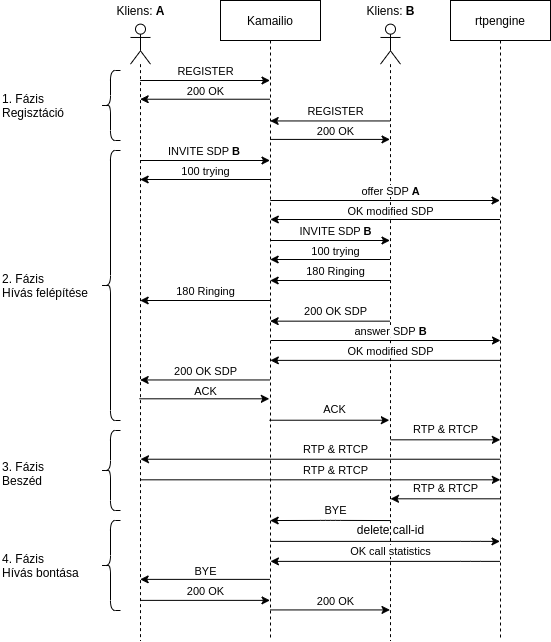
\includegraphics[width=0.9\textwidth, keepaspectratio]{figures/basic_call_flow.png}
	\caption{Kubernetes nélküli hívásfelépítés}
	\label{fig:callflow}
\end{figure}

Az \ref{fig:callflow} ábra segítségével a hívásfelépítés részeit.  Az ábrán látható 
egy teljes hívás folyamata a regisztrációtól egészen a hívás bontásáig. Négy részre 
bontottam a hívást annak érdekében, hogy könnyebb legyen a megértése.

Az első rész a regisztráció amelynek során a felhasználók csatlakoznak a SIP szerverhez.
Ilyenkor a kliens SIP REGISTER üzenetet küld a szervernek, amikkel hozzáadni, törölni és
lekérdezni lehet a felhasználó adait szerverről. Ha létezik a felhasználónak fiókja 
a szerveren, viszont még nem jelentkeztek be az adott eszközről akkor az első alkalommal 
egy 401 Unauthorized üzenettel tér vissza, ami felszólítja a klienst, hogy adja meg a 
hitelesítéshez szükséges felhasználói azonosítót és jelszót, amit egy újabb SIP REGISTER
üzenetben fog újraküldeni titkosítva. Ha minden megfelelt, akkor 200 OK üzenetet kap 
vissza a kliens, ami jelzi, hogy minden rendben és tud hívásokat kezdeményezni. Az ábrán
szereplő folyamat nem tartalmazza a 401-s üzenetet, mert már többször használva volt a 
kliens azon a virtuális gépen.

A következő rész pedig már a konkrét hívás kezdeményezése és felépítése. A hívást az 
\textbf{A} felhasználó kezdeményezi \textbf{B} irányába egy INVITE üzenettel, ami tartalmaz
egy SDP üzenetet is. Ez az SDP egy olyan protokoll, amivel a híváshoz kapcsolódó információkat
lehet továbbítani, mint például a támogatott média formátumok listája illetve a hívott fél
elérhetőségei. Mivel ebben az esetben \textbf{B} felhasználó címe létezik a szerveren így
a szerver 100 trying üzenettel jelzi \textbf{A}-nak, hogy elkezdte a hívást felépíteni. Erre
azért van szükség, hogy a kliens ne próbálkozzon újra a hívás felépítésével.

A szerver ilyenkor küld egy \textbf{offer} üzenetet az rtpengine felé, aminek legalább 
tartalmaznia kell az \textbf{A} által küldött SDP üzenetet, hívásazonosítót és a SIP üzenet
From mezőjét, ami az \textbf{A} azonosítója. Erre az rtpengine egy módosított SDP üzenetet küld
vissza a szervernek, amiben módosítja a cél címet és portot a sajátjára. Így minden RTP
üzenet elsőnek az rtpengine-hez fog elmenni és majd onnét megy tovább \textbf{B}-nek.

Ha ez is sikeresen megtörtént, a szerver átveszi a hívás kezdeményező szerepét a \textbf{B}-vel
szemben. Szóval küld egy INVITE üzenetet neki, amiben szerepel \textbf{A} azonosítója, de
a csatlakozást leíró mező az rtpengine címe lesz. A trying üzenet ebben az esetben is 
ugyan azt jelenti, mint mikor az \textbf{A} kezdeményezett. De itt már szerepel a 
\textbf{180 ringing}, amivel lehet jelzi, hogy feldolgozásra került az INVITE. Majd ugyan ez 
az üzenetet megkapja \textbf{A} is. 

Ha \textbf{B} elfogadta a hívást, akkor \textbf{200 OK}-l jelez a szervernek, amiből a
SIP szerver tudja, hogy \textbf{answer}-t kell küldenie az rtpengine felé, amivel a hívás teljesen
ki fog épülni az rtpengine-ben is. Az answer igazából ugyanazt a funkciót valósítja meg,
mint az offer. Mivel az rtpengine kapott offer-t és answer-t is, így a hívást kiépítheti
és az előzőleg lefoglalt négy porton képes fogadni a forgalmat, amit feldolgozva 
tovább küld. Azért foglal le négy port, mert felenként kell egy páros számú port az 
RTP forgalomnak és egy páratlan számú az RTCP-nek. Végül pedig egy SIP ACK üzenettel van
értesítve mind a két fél arról, hogy a hívás sikeresen kiépült és elkezdhetnek 
beszélni. 

Mivel már létezik a hívás így már lehet küldeni a forgalmat az rtpengine adott 
portjaira. Ahol a legegyszerűbb esetben annyi történik, hogy az \textbf{A}-hoz rendelt
RTP porton kapott csomagokat kiküldi a \textbf{B}-hez a hozzárendelt portról. Ugyanez
történik RTCP esetében is. 

Mikor vége a hívásnak, akkor megkezdődik a hívás lebontása egy BYE SIP üzenettel. Aminek
hatására a SIP szerver egy delete üzenetet ad ki az rtpengine felé, ami tartalmazza a hívás
azonosítóját. Ekkor törlődik minden a híváshoz kapcsolódó információ és a számukra kinyitott
portok is lezárnak. De a rtpengine válaszában szerepelnek a hívásról információk, amik alapján
könnyen lehet statisztikákat készíteni például a hívások átlagos hosszáról vagy minőségéről.